\begin{longtable}{p{0.5\textwidth} p{0.5\textwidth}}
  \tablesection{Appendix I: Supplementary Information}
  \tablesubsection{Lagrange Point Calculations}
   & \\%hopefully spaces stuff nicely
\end{longtable}
%==========================
%==== Lagrange Diagram ====
%==========================

\begin{figure}[h]%positions figure after longtable env.
  \centering
  \begin{tikzpicture}[scale=\textwidth]

    %creates m1, m2, and L
    \node (m1) [circle, draw=black, fill=white, text=black,
    scale=3]{$M_1$};%draws M1
    \node (m2) [circle, draw=black, fill=white,
    text=black, scale=1.5, right=0.5\textwidth of m1]{$M_2$};%draws M2
    \node (L) [draw=white, fill=white, text=black, left=1.5 of m2]{\textbullet};%draws point L
    \node [draw=white, fill=white, text=black, below=0.01 of L]{$L$};%labels point L

    %draws lines for x and R-x
    \draw (m1) to node[midway, below, sloped]{$R-x$} (L);%draws R-x
    \draw (m2) to node[midway, below, sloped]{$x$} (L);%draws x

    %draws brace for R
    \draw [decorate, decoration={brace, amplitude=10pt, raise=5pt}] (m1) to node[midway, yshift=25pt, sloped]{$R$} (m2);%draws R (yshift is relative to line y=0)
  \end{tikzpicture}

  \caption{A diagram of two large masses $M_1$ and $M_2$ separated by distance $R$ with the lagrange point $L$ between them at the point where the force of gravity for each mass is equivalent ($F_{GM_1} = F_{GM_2}$)}
  \label{fig:lagrange_diag}
\end{figure}

%==========================
%===== Lagrange Math ======
%==========================

The Lagrange point $L$ is located at the equilibrium point for the forces of gravity for each mass. We want to find the distance of that point from the mass $M_2$.
\begin{equation*}
	F_{G,1} = F_{G,2} 
\end{equation*}

Given $F_{G,1} = F_{G,2}$, rewrite the equation for the equilibrium point. Assume the Lagrange point $L$ is $M_L$ of negligible mass.
\begin{equation*}
	G \displaystyle\frac{M_1 M_L}{r_{L,1}^2} = G\frac{M_L M_2}{r_{L,2}^2}
\end{equation*}

Replace each $r$-value with the components of $R$, those being $x$ and $R-x$, from the diagram above and cancel out shared terms as follows.
\begin{equation*}
	\displaystyle\frac{M_1}{\left(R-x\right)^2} = \frac{M_2}{x^2}
\end{equation*}

Finally, algebraically rearrange the formula to yield $x$, the distance between $L$ and $M_2$.
\begin{equation*}
	x = \frac{R}{\sqrt{\frac{m_1}{m_2}} + 1} 
\end{equation*}

\textbf{N.B.} Instruction on this material in class was especially unclear. It is advised that you perform additional research on this topic at resources like \url{http://en.wikipedia.org/wiki/Lagrangian_point} before relying on this appendix item. The authors are of the impression that the example on this page is meant for the calculation of $L_1$.

% Diagram of points <-- this might be causing the compiler to run out of time on overleaf
%\begin{figure}[p]
%  \centering
%  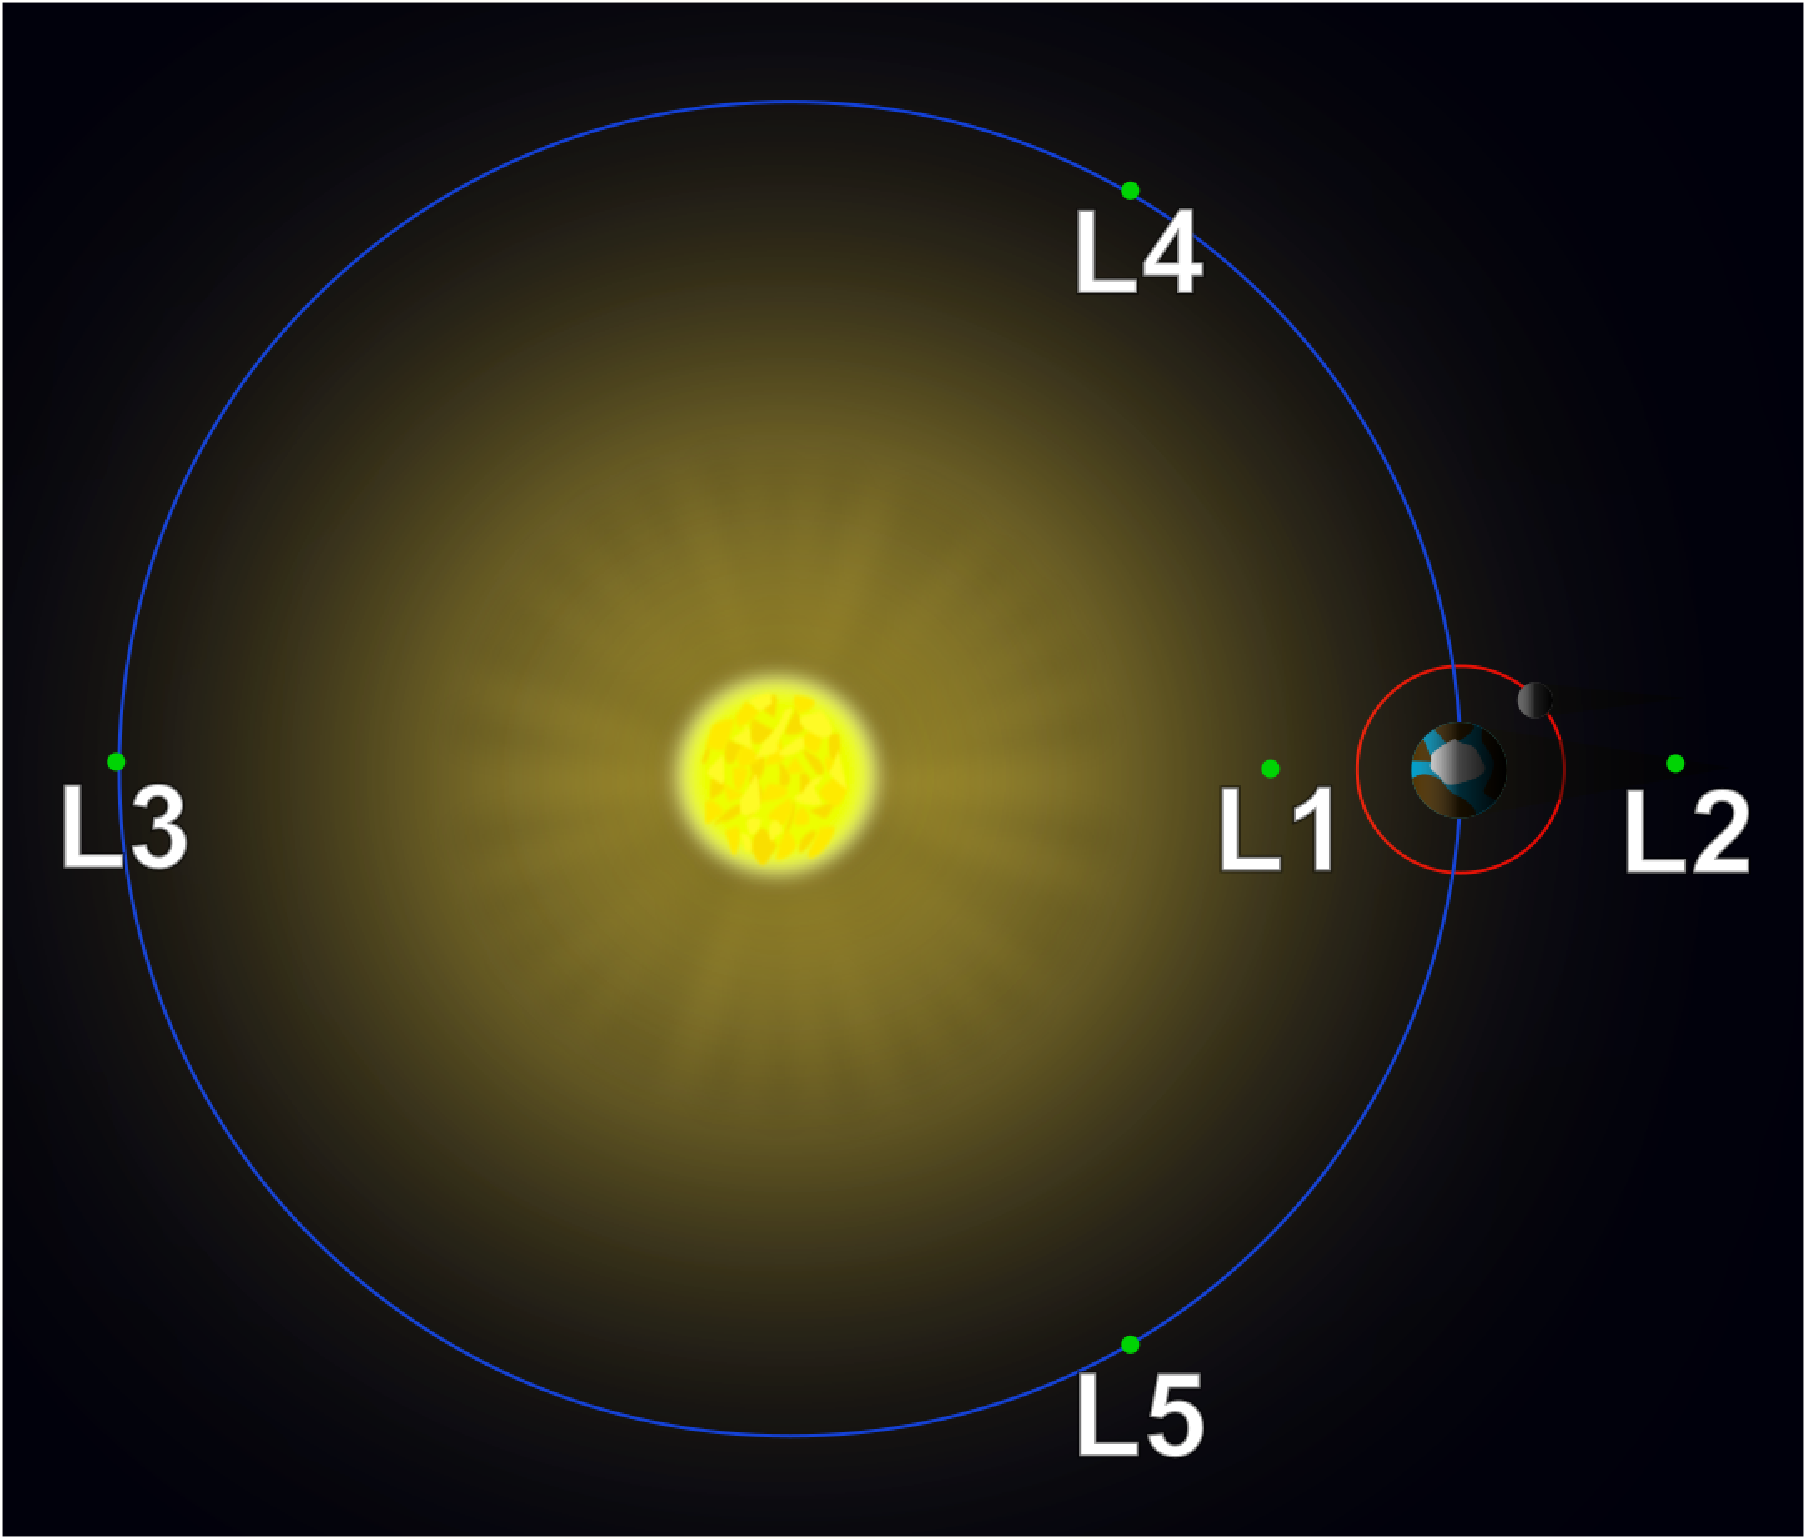
\includegraphics[width=\textwidth]{appendix-01/Lagrange_Points_Diagram} \vfill
%  \caption{A diagram of the five Langrangian points in the Moon--Earth--Sun system.}
%  \label{fig:lagrange_five}
%\end{figure}

%%% Local Variables:
%%% mode: latex
%%% TeX-master: "main"
%%% End: